\documentclass{book}
\usepackage{graphicx}
\graphicspath{{./images}}
\begin{document}
\chapter{Active Galaxies}
\section{Introduction}

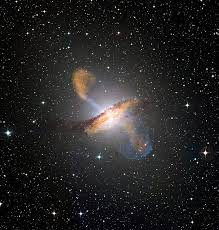
\includegraphics{agn.jpeg}


Between 2\% to 10\% of all the galaxies have active nuclei. The nucleus is bright, compact and sometimes brighter than the entire galaxy. The spectrum differs, too, showing strong, brouad emission lines arising from the hot and dense. highy excited gas.
\bigskip


These AGN are also variable on short time scales of about one or two days to show variations. This means that whatever is making the variation is small.
	
	In general, 30-50\% of spiral galaxies show some level of activity in their nuclei, but only about 10\% are truly dominant.  



There are various types of active galaxies;
\begin{enumerate}
\item Syfert Galaxies
\item Radio Galaxies
\item Quasars
\item blazars
\end{enumerate}

\section{Syfert Galaxies}
Syfert galaxies shows brouad emission lines (along with the normal absorbtion spectrum) which indicates the presencs of hot low-density gas.

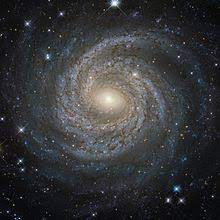
\includegraphics{syfert.jpeg}


Lines are broad which indicates that gas is in rapid rotation.
Gas moving towards us give rise to blue shifted lines and gas moving away gives rise to red shifted lines and the combination (result) gives the broad lines in the spectrum.

Ionised gas in the nuclei of syfert galaxies moves with a speed 30 times greater than that observed in normal galaxies.

Syfert is categorised into two types;
\begin{enumerate}
\item Type-1 syfert
\item Type-2 syfert
\end{enumerate}

\subsection{Type-1 syfert}
This has narrow emission features on top of broad emission lines.

\subsection{Type-2 syfert}
This just shows narrow lines.


\section{Radio Galaxies}
These galaxies also emit radio waves.
Big radio lobes are outside the boundary of the galaxy.


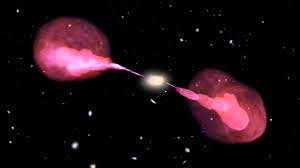
\includegraphics{radio.jpeg}


Lobes are more often in pairs.
These Lobes were associated with galaxies with Active Galactic Nuclei.

Galaxies with this property are often known as \textbf{Double-Lobed Radio Sources}.

Particles get accelerated close to speed of light and get shot out to both the sides of the galaxy, hit something outside the galaxy and form big diffused lobes of radio energy.


\section{Quasars}
These are most energetic objects in the universe.
Extreme brightness of quasars can fluctuate over day long periods, which indicates that the source of the energy is not more than a few light days across, incredibly tiny compared to the size of galaxy.


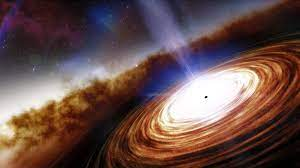
\includegraphics{quasar.jpeg}


When first seen, their spectrum was highly red-shifted which made to conclude that they are not in our galaxy and are much far away.

They shoot jets which travel with a speed close to speed of light.


\section{Blazars}
They are light quasars.

When jets point towards the earth, it is considered a blazar.


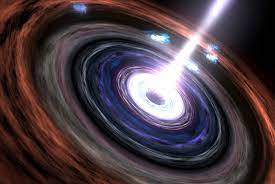
\includegraphics{blazar.jpeg}

\end{document}

